\documentclass[border=10pt]{standalone}

\usepackage{tikz}
\usepackage{tikzsymbols}
\usetikzlibrary{calc,patterns,shapes.geometric}

\def\centerarc[#1](#2)(#3:#4:#5){\draw[#1] ($(#2)+({#5*cos(#3)},{#5*sin(#3)})$) arc (#3:#4:#5);}

\begin{document}
	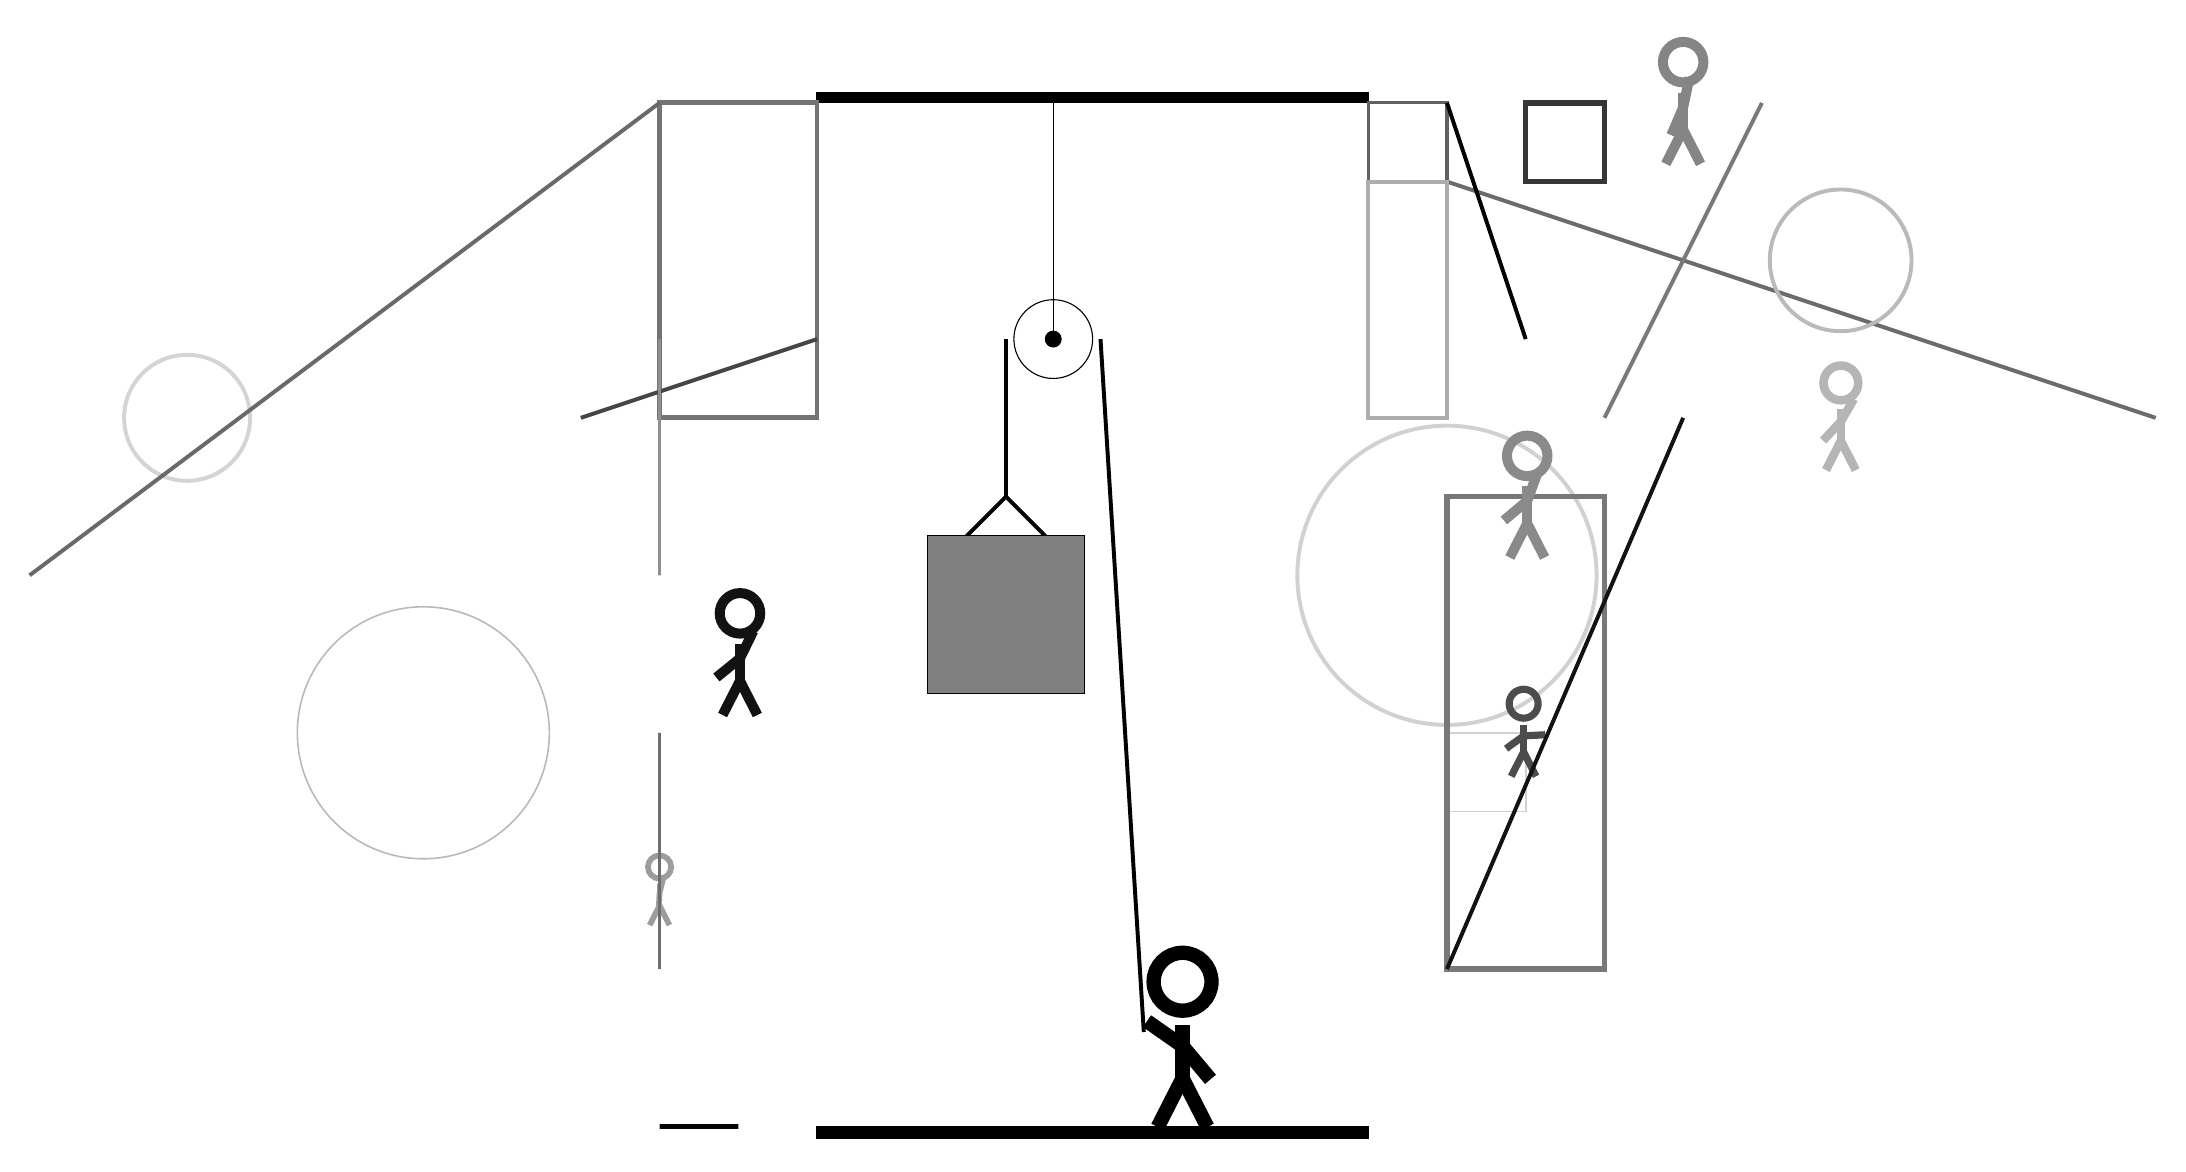
\begin{tikzpicture}
		%%%%% START %%%%%
		
		\draw[fill=black] (-2, 10) rectangle (5, 10.125);
		
		\draw (1, 7) circle (0.5);
		\draw[fill=black] (1, 7) circle (0.1);
		\draw (1, 10) -- (1, 7);
		
		\draw[line width=0.5mm] (-0.1, 4.5) -- (0.4, 5.0) -- (0.9, 4.5);
		\draw[fill=black!50] (-0.6, 4.5) rectangle (1.4, 2.5);
		
		\draw[line width=0.5mm] (0.4, 7) -- (0.4, 5.0);
		\centerarc[line width=0.5mm](1, 7)(0:180:0.6);
		\draw[line width=0.5mm](1.6, 7) -- (2.15, -1.8);
		
		\draw[line width=0.4mm, color=black!62] (6, 6) rectangle (5, 10);
		
		\draw[line width=0.5mm, color=black!58](6, 9) -- (15, 6);
		\draw[line width=0.2mm, color=black!18] (7, 1) rectangle (6, 2);
		\draw[line width=0.5mm, color=black!99](7, 7) -- (6, 10);
		\node[line width=0.7mm, color=black!29] at (11, 6) {\Strichmaxerl[6][47][60]};
		\node[line width=0.6mm, color=black!48] at (9, 10) {\Strichmaxerl[7][67][78]};
		\draw [line width=0.5mm, color=black!18](6, 4) circle (1.9);
		\draw[line width=0.7mm, color=black!98] (-4, -3) rectangle (-3, -3);
		\draw [line width=0.5mm, color=black!17](-10, 6) circle (0.8);
		\draw[line width=0.5mm, color=black!32] (6, 6) rectangle (5, 9);
		
		\draw[line width=0.6mm, color=black!55] (-2, 6) rectangle (-4, 10);
		\node[line width=0.3mm, color=black!70] at (7, 2) {\Strichmaxerl[5][36][3]};
		\draw[line width=0.5mm, color=black!73](-5, 6) -- (-2, 7);
		
		\draw [line width=0.2mm, color=black!28](-7, 2) circle (1.6);
		\draw[line width=0.7mm, color=black!53] (6, 5) rectangle (8, -1);
		\node[line width=0.4mm, color=black!93] at (-3, 3) {\Strichmaxerl[7][39][64]};
		
		\draw[line width=0.7mm, color=black!79] (7, 10) rectangle (8, 9);
		\node[line width=0.2mm, color=black!39] at (-4, 0) {\Strichmaxerl[4][87][76]};
		\node[line width=0.3mm, color=black!46] at (7, 5) {\Strichmaxerl[7][40][70]};
		\draw[line width=0.5mm, color=black!59](-4, 10) -- (-12, 4);
		\draw[line width=0.5mm, color=black!53](8, 6) -- (10, 10);
		
		\draw[line width=0.3mm, color=black!57] (-4, -1) rectangle (-4, 2);
		\draw[line width=0.3mm, color=black!44] (-4, 7) rectangle (-4, 4);
		\draw [line width=0.5mm, color=black!27](11, 8) circle (0.9);
		\draw[line width=0.5mm, color=black!93](6, -1) -- (9, 6);
		
		\node at (2.6, -1.9) {\Strichmaxerl[10][-35][-50]};
		
		\draw[fill=black] (-2, -3) rectangle (5, -3.15);
		
		%%%%% END %%%%%
	\end{tikzpicture}
\end{document}